% q2.tex - Question 2 (OWNER: A) - revised from docs/A_Q2.md
\section{Question 2: Which Feed Helps Chicks Grow?}

The \texttt{chickwts} dataset is complete with 71 observations and no missing values on either variable. All 71 chicks were retained in the analysis; the residual degrees of freedom ($65 = 71 - 6$) confirm that the full sample entered the model.

\FloatBarrier
\subsection*{(a) Hypotheses and assumptions}

Let $\mu_i$ denote the population mean of the body weight of chicks after six weeks of being fed the feed $i$ ($i =$ casein, horsebean, linseed, meatmeal, soybean, sunflower).

\[
\Hnull\colon \mu_1 = \mu_2 = \mu_3 = \mu_4 = \mu_5 = \mu_6
\]
\[
\Halt\colon \text{At least one feed has a different population mean. } (\alpha = 0.05)
\]

Three main assumptions apply.

\textbf{Independence:} The observations should not influence one another, within or between groups. This assumption is supported by the study design rather than by a statistical test: newly hatched chicks were randomly allocated to the six feed groups, and each chick is an independent experimental unit.

\textbf{Normality:} The weights within each feed group should be approximately normally distributed. This is assessed from the data: a Shapiro--Wilk test on the ANOVA residuals gives $W = 0.986$, $\pval = 0.627$, and the residual Q--Q plot (Figure Q2-2) shows the points lying close to the reference line with no systematic departure. Approximate normality is therefore reasonable.

\textbf{Homogeneity of variance:} The six population variances should be equal. This is checked with Levene's test centred on group medians (the default in the \texttt{car} package), $F(5, 65) = 0.749$, $\pval = 0.590$; the mean-centred version gives $F = 0.987$, $\pval = 0.432$, with the same conclusion. Neither version rejects equal variances.

The design and diagnostics provide reasonable support for a one-way ANOVA; non-significant diagnostic tests do not prove that its assumptions hold exactly.

\FloatBarrier
\subsection*{(b) Plot, ANOVA table and decision}

\begin{table}[htbp]
  \centering
  \caption*{Table Q2-1: One-way ANOVA of six-week chick weight by feed supplement.}
  \begin{tabular}{lrrrrl}
    \toprule
    Source & df & SS & MS & $F$ & $\pval$ \\
    \midrule
    Feed & 5 & 231129 & 46226 & 15.365 & $< 0.001$ \\
    Residuals & 65 & 195556 & 3009 & & \\
    Total & 70 & 426685 & & & \\
    \bottomrule
  \end{tabular}
\end{table}

Figure Q2-1 (labelled boxplot of weight by feed) shows the highest weights under casein and sunflower and clearly lower weights under horsebean. The one-way ANOVA table (Table Q2-1) gives SS(feed) $= 231129$ on 5 df, SS(residuals) $= 195556$ on 65 df, MS(feed) $= 46226$, MS(residuals) $= 3009$, $F(5, 65) = 15.365$ with $\pval < 0.001$. Since $\pval < 0.05$ we reject $\Hnull$ and conclude that the six feed types do not all have the same population mean chick weight after six weeks; feed explains about 54.2\% of the variation in weight ($R^2 = \text{SS(feed)}/\text{SS(total)} = 231129/426685 = 0.542$). Which particular feeds differ would require post-hoc comparisons, which are beyond the required scope.

\begin{figure}[htbp]
  \centering
  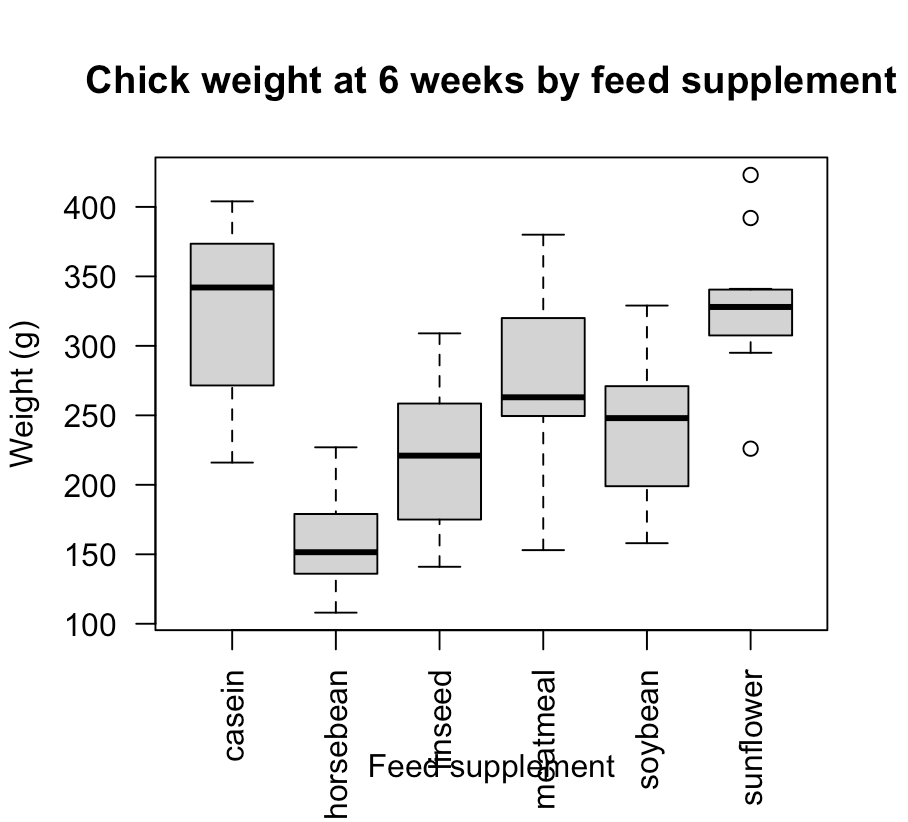
\includegraphics[width=0.75\textwidth]{Q2-1_boxplot.png}
  \caption*{Figure Q2-1: Labelled boxplot of chick weight by feed supplement.}
\end{figure}

\begin{figure}[htbp]
  \centering
  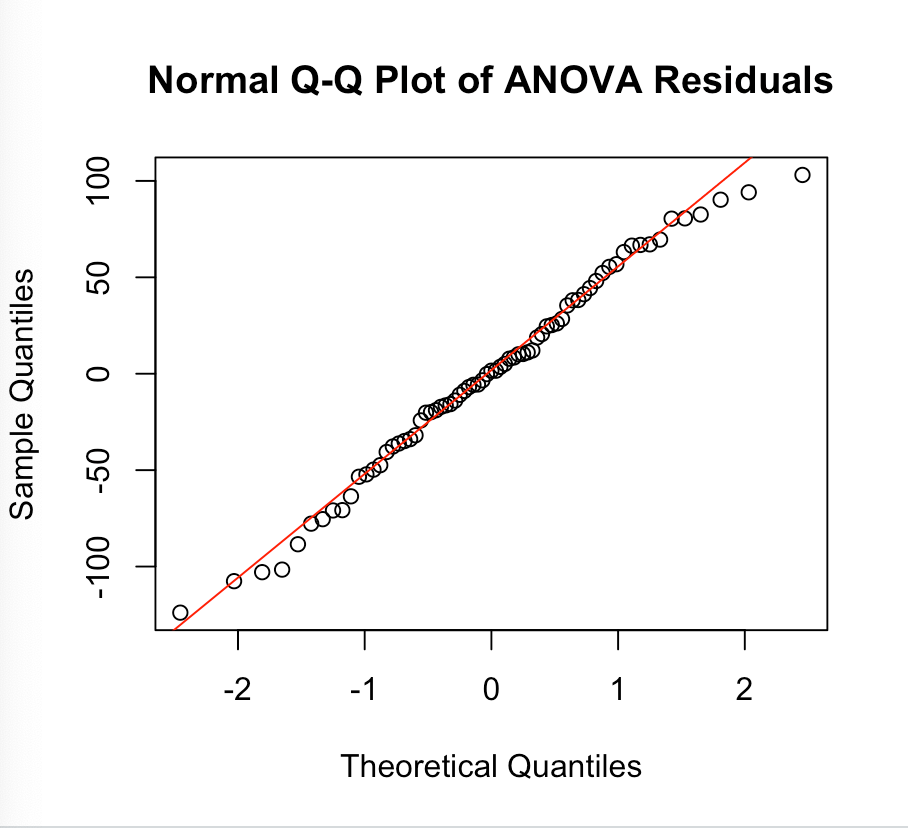
\includegraphics[width=0.6\textwidth]{Q2-2_qqplot.png}
  \caption*{Figure Q2-2: Residual Q--Q plot for the one-way ANOVA.}
\end{figure}

\FloatBarrier
\subsection*{(c) Interpretation of the claim}

This argument does not hold. A significant ANOVA F-test is an omnibus result: it only rejects the null hypothesis that ``all six population means are equal,'' establishing that ``at least one feed is different,'' but it does not establish that ``each feed is different from every other feed.'' For example, a data pattern where ``five feeds share the same mean and only one is lower'' would also yield a significant F-statistic.

The highest sample mean does not imply that it is significantly superior to all other groups: sunflower (328.9 g) exceeded casein (323.6 g) by only 5.3 g, while within-group variation is substantial. This descriptive ranking alone does not establish a statistically significant pairwise difference.

A reliable conclusion that can be drawn from this analysis is that the average weights of the six feeds are not all equal ($F(5, 65) = 15.365$, $\pval < 0.001$); descriptive evidence indicates that the weight for horsebean is lower, while those for sunflower and casein are higher. To identify which specific pairings differ, we would need to perform post-hoc multiple comparisons, such as Tukey's HSD, which controls the family-wise error rate across all 15 pairwise comparisons; however, this is not required for this problem.
